\documentclass[11pt]{article}
\usepackage{graphicx}
\usepackage{subcaption}
\usepackage{tabularx}
\usepackage{float}
\usepackage{listings}
\usepackage{caption}
\usepackage{amsmath}
\usepackage{amssymb}
\usepackage{listings}
\usepackage[inline]{enumitem}
\usepackage{xcolor}
\usepackage[top = 0.7in,bottom = 0.8in, left = 0.8in, right = 0.8in]{geometry} 

%New colors defined below
\definecolor{codegreen}{rgb}{0,0.6,0}
\definecolor{codegray}{rgb}{0.5,0.5,0.5}
\definecolor{codepurple}{rgb}{0.58,0,0.82}
\definecolor{backcolour}{rgb}{0.95,0.95,0.92}

%Code listing style named "mystyle"
\lstdefinestyle{mystyle}{
  backgroundcolor=\color{backcolour},   commentstyle=\color{codegreen},
  keywordstyle=\color{magenta},
  numberstyle=\tiny\color{codegray},
  stringstyle=\color{codepurple},
  basicstyle=\ttfamily\footnotesize,
  breakatwhitespace=false,         
  breaklines=true,                 
  captionpos=b,                    
  keepspaces=true,                 
  numbers=left,                    
  numbersep=5pt,                  
  showspaces=false,                
  showstringspaces=false,
  showtabs=false,                  
  tabsize=2
} 
\lstset{style=mystyle}

\title{\textbf{SC651 : Assignment 1}}
\author{\textbf{Adityaya Dhande}   \hspace{8mm} \textbf{210070005}}
\date{}
\begin{document}
\maketitle
\section{Numerical integrators}
I have simulated the spring-mass system without a damper to better study the performances of different 
numerical integrators. I implemented the four different numerical integration methods -- \textbf{Forward Euler}, \textbf{Backward Euler},
\textbf{Symmetric Euler}, \textbf{Symplectic Euler} for both the Spring-Mass and Vertical Pendulum system. I also evaluated the analytical solution for
the Spring-Mass system and used it to analyse the performances of the different numerical methods. 
 
\subsection*{Spring-Mass system : Analysis with varying time-steps}
\begin{table}[H]
    \begin{center}
        \caption*{Variation of \textbf{absolute average error (in metres)} with $\Delta T$}
        \begin{tabular}{|c|c|c|c|c|}
            \hline
             $\Delta T (s)$ &  Forward & Backward & Symmetric & Symplectic \\
            \hline
            0.1   &  0.6153 & 0.2703   &  0.0134 & 0.0353\\
            \hline
            0.01   &  0.0412 & 0.0379   &  0.0001 & 0.0032\\
            \hline   
            0.001   &  0.0040 & 0.0039   &  1.34e-6 & 0.0003\\
            \hline     		
        \end{tabular}
    \end{center}
 \end{table}
The solution obtained using \textbf{Forward Euler} grows unbounded and the solution obtained using \textbf{Backward Euler}
dies down over time, as opposed to the original solution which is sinusoidal and does not grow unbounded with time. The performance of 
\textbf{Symmetric Euler} and \textbf{Symplectic Euler} is significantly better. The error of Symplectic Euler solution is intially higher than that of Symmetric Euler, but the error of Symmetric Euler solution grows at a faster rate.
\begin{figure}[H]
    \centering
    \begin{subfigure}[H]{0.49\linewidth}
      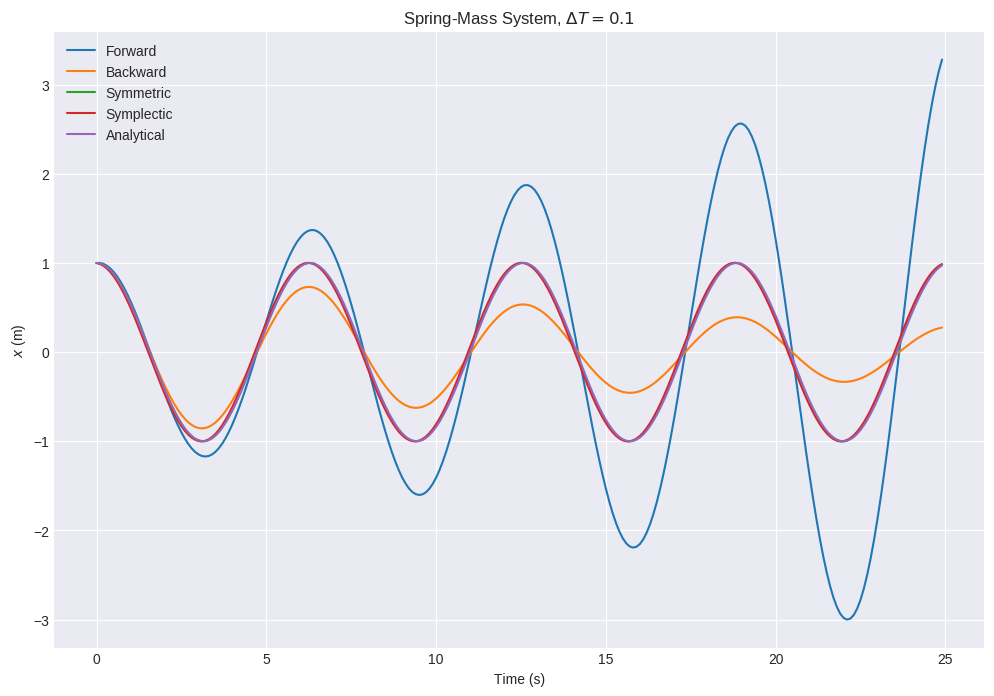
\includegraphics[width=\linewidth]{../sm1.png}
      \caption*{Position vs Time}
    \end{subfigure}
    \begin{subfigure}[H]{0.49\linewidth}
      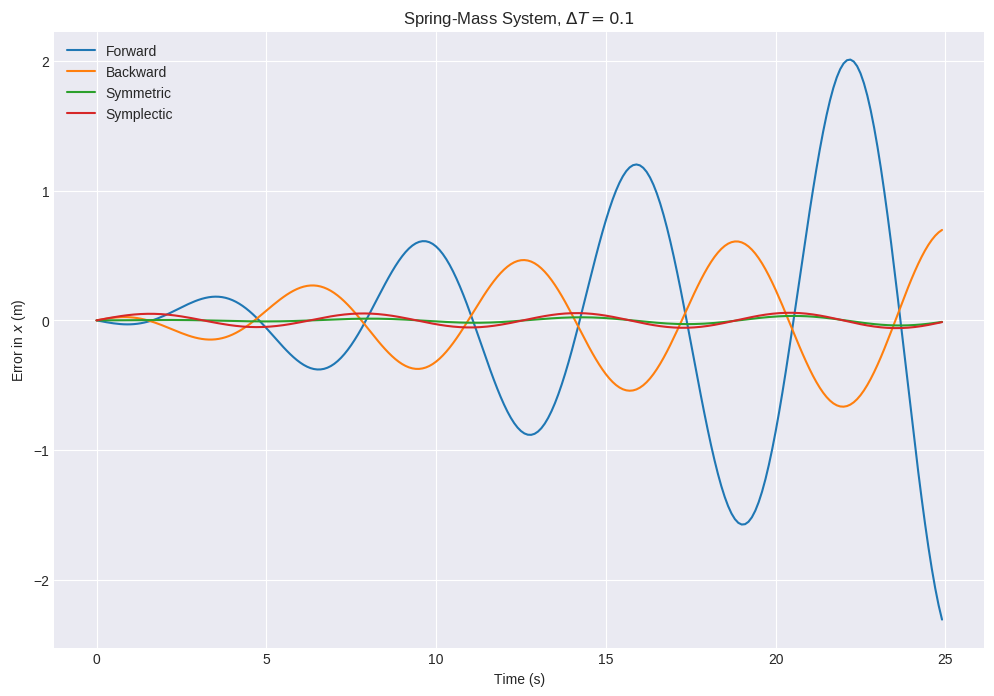
\includegraphics[width=\linewidth]{../sm2.png}
      \caption*{Error vs Time}
    \end{subfigure}
    \caption*{Spring-Mass system, $\Delta T = 0.1s$}
  \end{figure}

\begin{figure}[H]
    \centering
    \begin{subfigure}[H]{0.49\linewidth}
        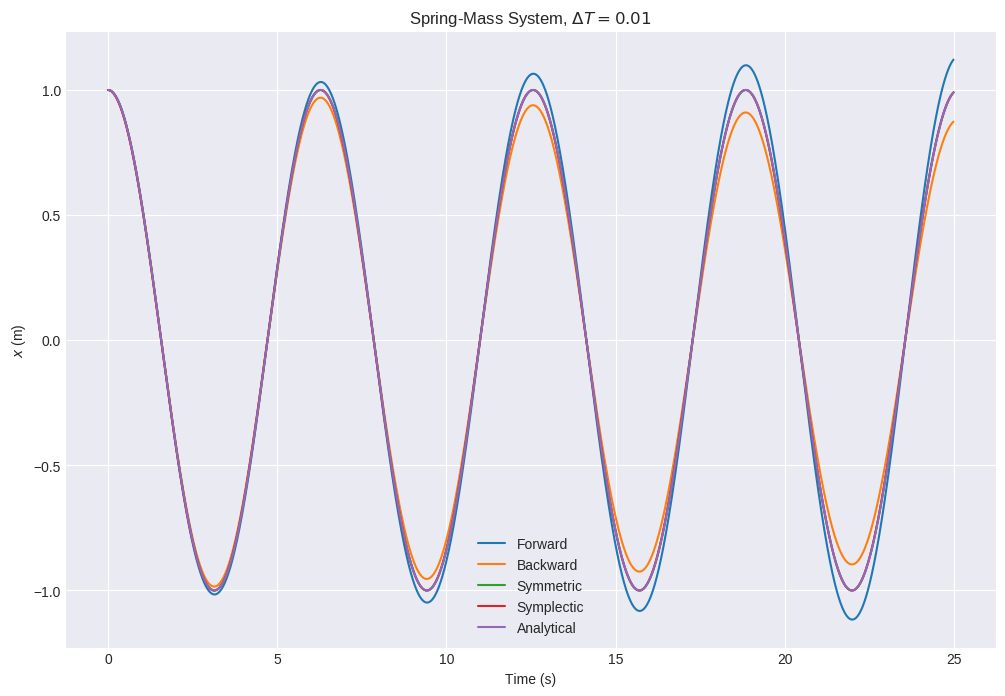
\includegraphics[width=\linewidth]{../sm3.png}
        \caption*{Position vs Time}
    \end{subfigure}
    \begin{subfigure}[H]{0.49\linewidth}
        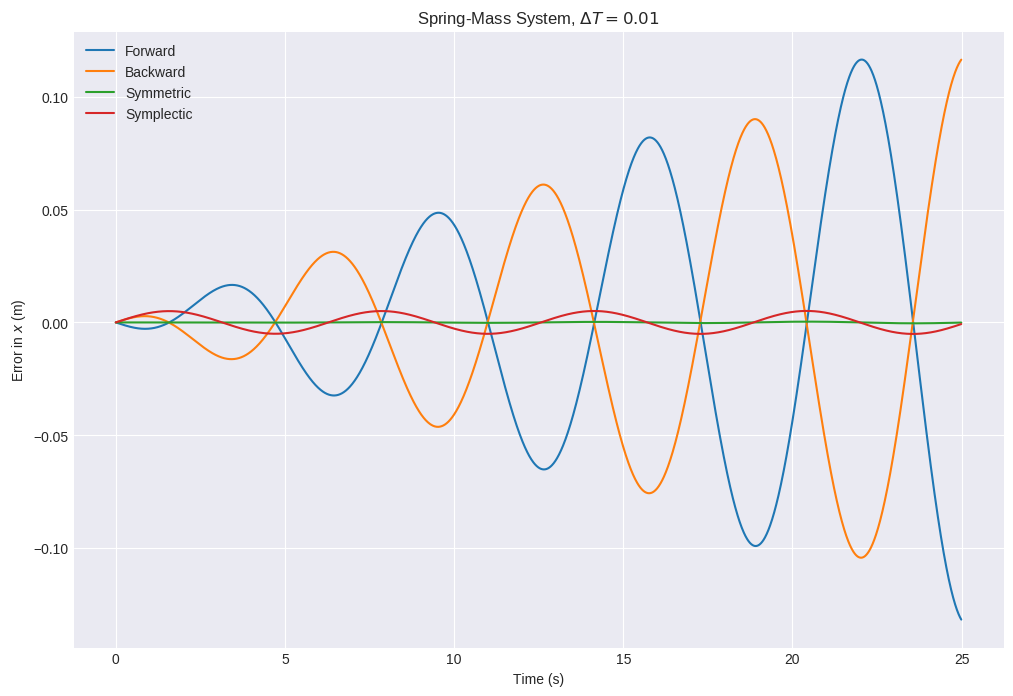
\includegraphics[width=\linewidth]{../sm4.png}
        \caption*{Error vs Time}
    \end{subfigure}
    \caption*{Spring-Mass system, $\Delta T = 0.01s$}
    \end{figure}

\begin{figure}[H]
    \centering
    \begin{subfigure}[H]{0.49\linewidth}
        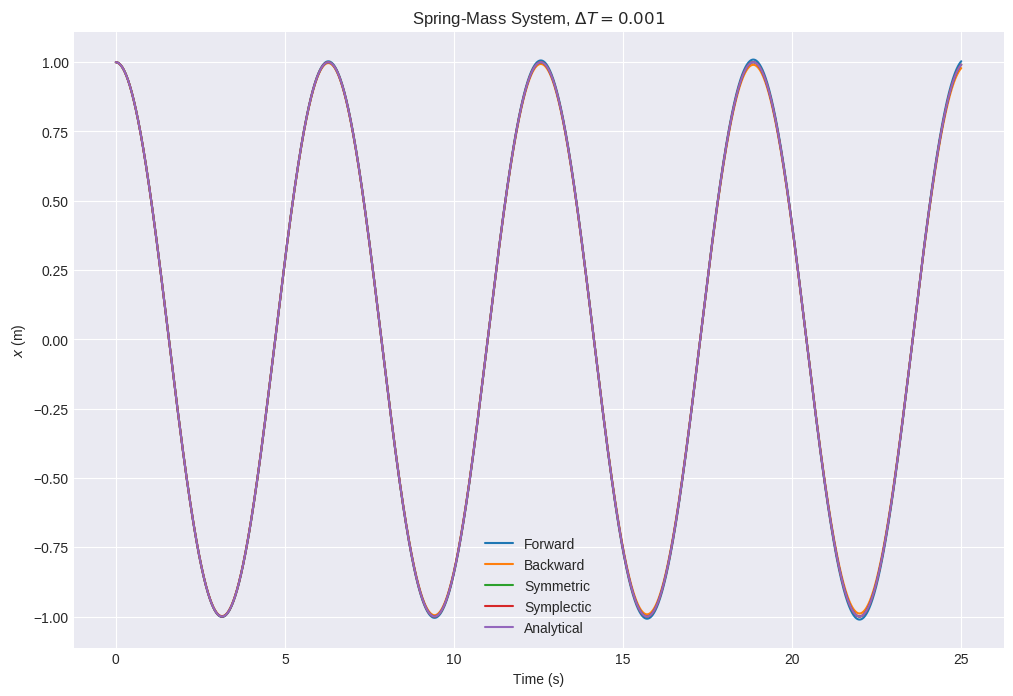
\includegraphics[width=\linewidth]{../sm5.png}
        \caption*{Position vs Time}
    \end{subfigure}
    \begin{subfigure}[H]{0.49\linewidth}
        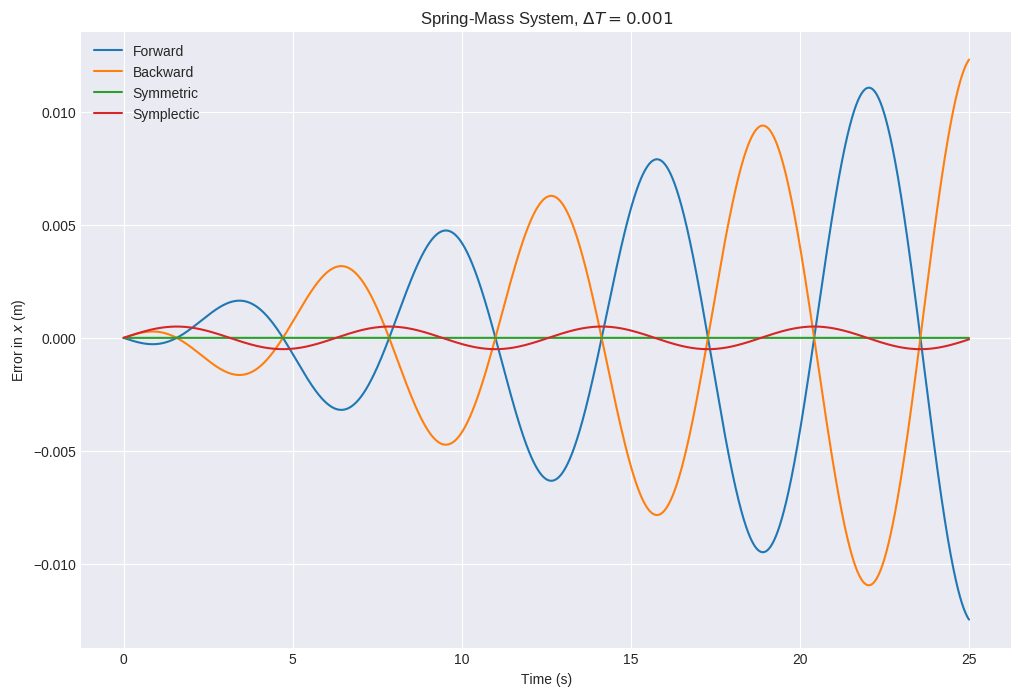
\includegraphics[width=\linewidth]{../sm6.png}
        \caption*{Error vs Time}
    \end{subfigure}
    \caption*{Spring-Mass system, $\Delta T = 0.001s$}
    \end{figure}

\begin{figure}[H]
    \centering
    \begin{subfigure}[H]{0.49\linewidth}
        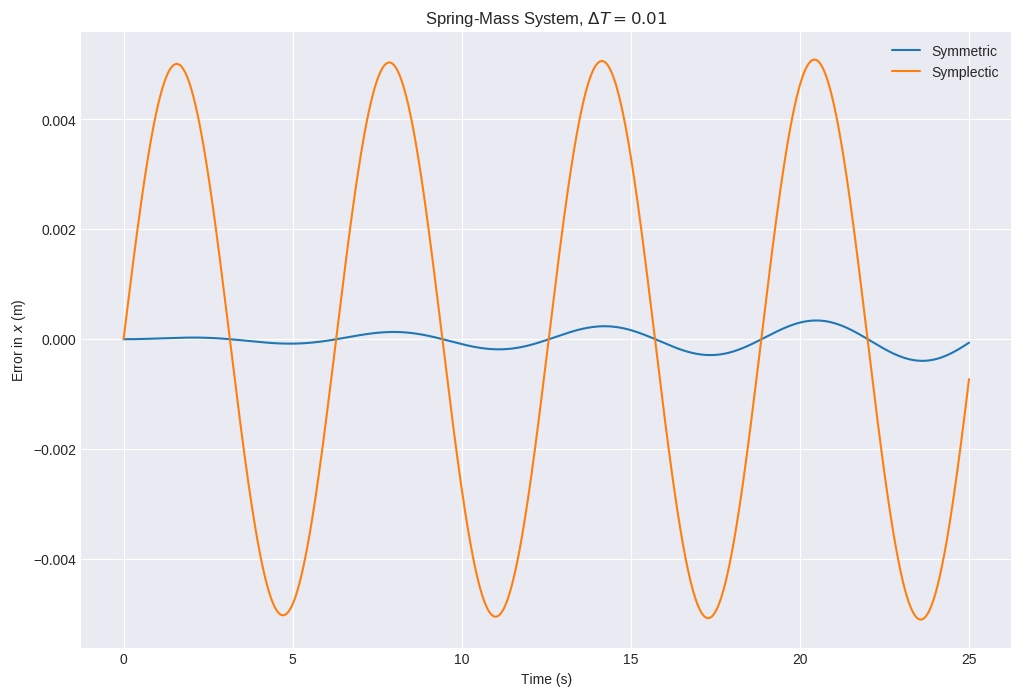
\includegraphics[width=\linewidth]{../sm7.png}
        \caption*{$\Delta T = 0.01s$}
    \end{subfigure}
    \begin{subfigure}[H]{0.49\linewidth}
        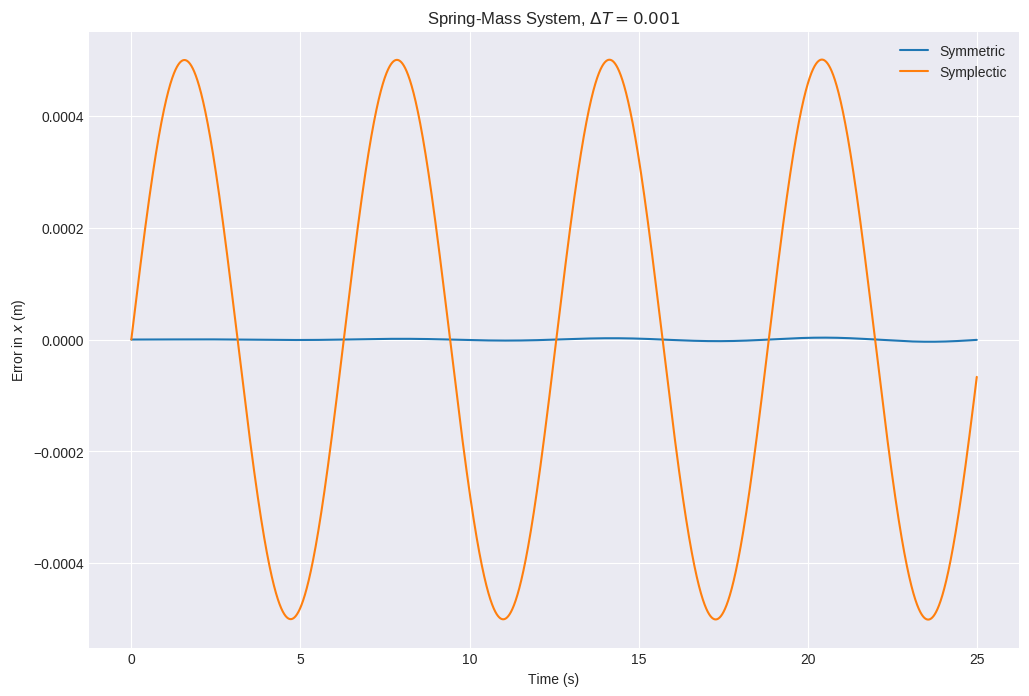
\includegraphics[width=\linewidth]{../sm8.png}
        \caption*{$\Delta T = 0.001s$}
    \end{subfigure}
    \caption*{Error of Symplectic and Symmetric Euler}
    \end{figure}

    

\subsection*{Sping-Mass system : Analysis with varying time horizon}
\begin{table}[H]
    \begin{center}
        \caption*{Variation of \textbf{absolute average error (in metres)} with horizon}
        \vspace{2mm}
        \begin{tabular}{|c|c|c|c|c|}
            \hline
             Horizon $(s)$ &  Forward & Backward & Symmetric & Symplectic \\
            \hline
            200  &  0.4556 & 0.2336   &  0.0011 & 0.0035\\
            \hline
            500   &  2.2141 & 0.4031   &  0.0026 & 0.0038\\
            \hline   
            1000   &  18.1593 & 0.5104   &  0.0053 & 0.0045\\
            \hline     		
        \end{tabular}
    \end{center}
 \end{table}

 \textbf{Forward} and \textbf{Backward Euler} perform very poorly for large horizons. The 
 error due of \textbf{Symmetric Euler} solution is lower than that of \textbf{Symplectic Euler} initially but 
 it grows at a faster rate and Symplectic Euler performs better at larger horizons.
For the given system, $\ddot{x} + x = 0$, all the numerical solutions diverge with time.
\begin{figure}[H]
    \centering
    \begin{subfigure}[H]{0.49\linewidth}
      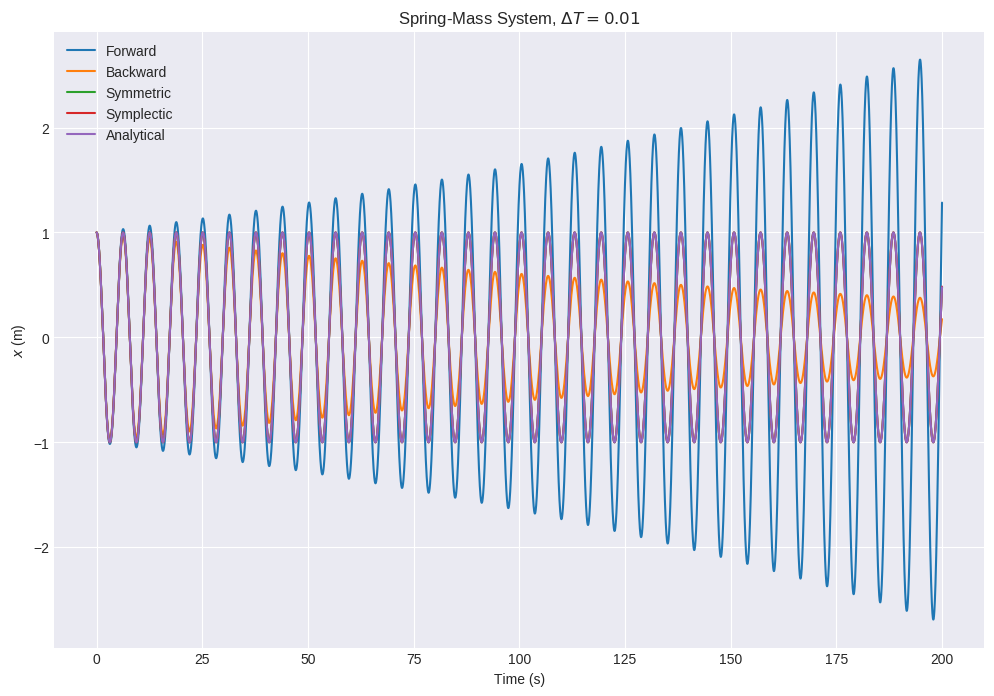
\includegraphics[width=\linewidth]{../sm9.png}
      \caption*{Position vs Time}
    \end{subfigure}
    \begin{subfigure}[H]{0.49\linewidth}
      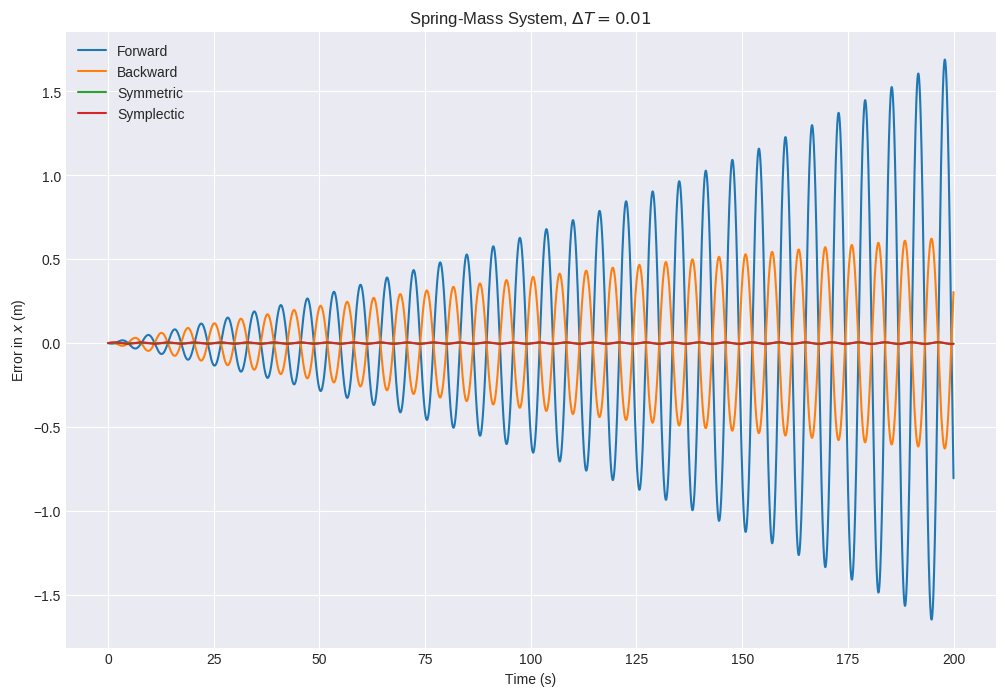
\includegraphics[width=\linewidth]{../sm10.png}
      \caption*{Error vs Time}
    \end{subfigure}
    \caption*{Spring-Mass system, Horizon$ = 200s$}
  \end{figure}

\begin{figure}[H]
    \centering
    \begin{subfigure}[H]{0.49\linewidth}
        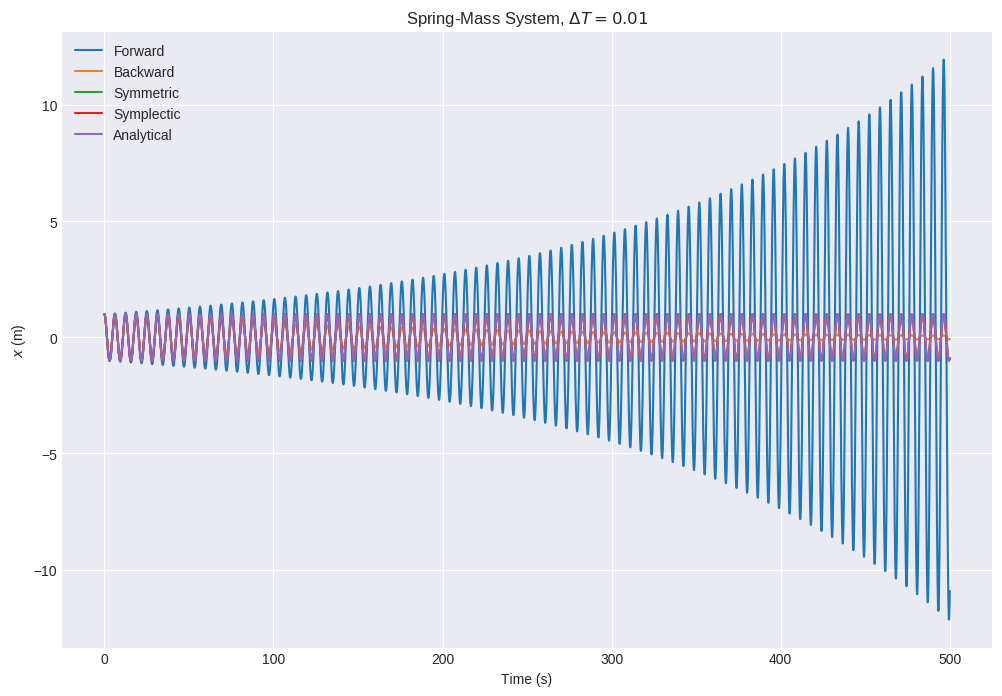
\includegraphics[width=\linewidth]{../sm12.png}
        \caption*{Position vs Time}
    \end{subfigure}
    \begin{subfigure}[H]{0.49\linewidth}
        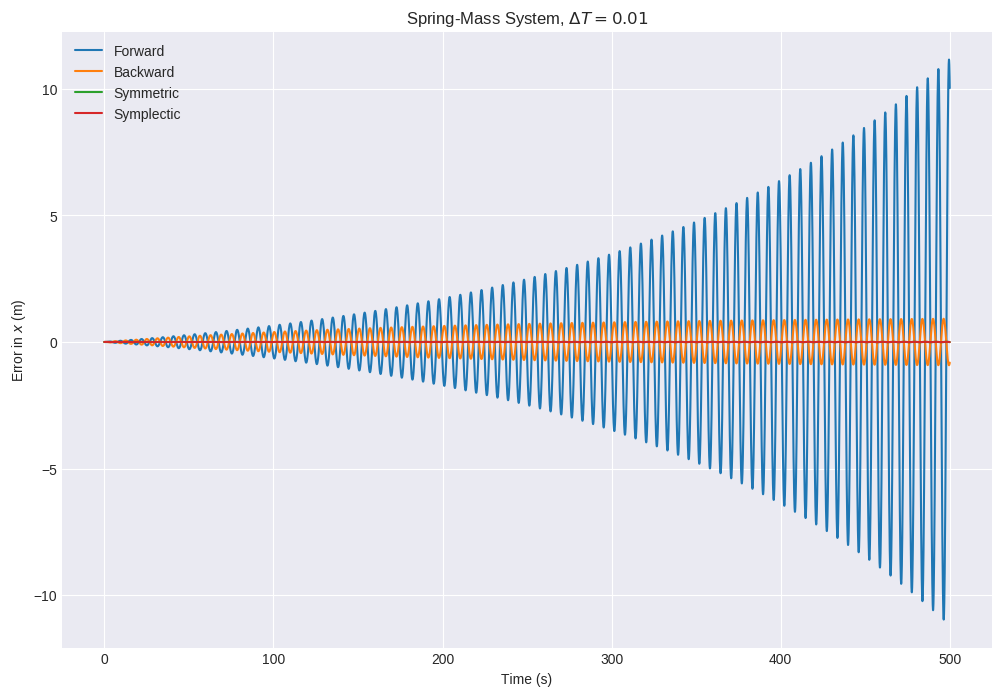
\includegraphics[width=\linewidth]{../sm14.png}
        \caption*{Error vs Time}
    \end{subfigure}
    \caption*{Spring-Mass system, Horizon$ = 500s$}
    \end{figure}

    \begin{figure}[H]
        \centering
        \begin{subfigure}[H]{0.49\linewidth}
            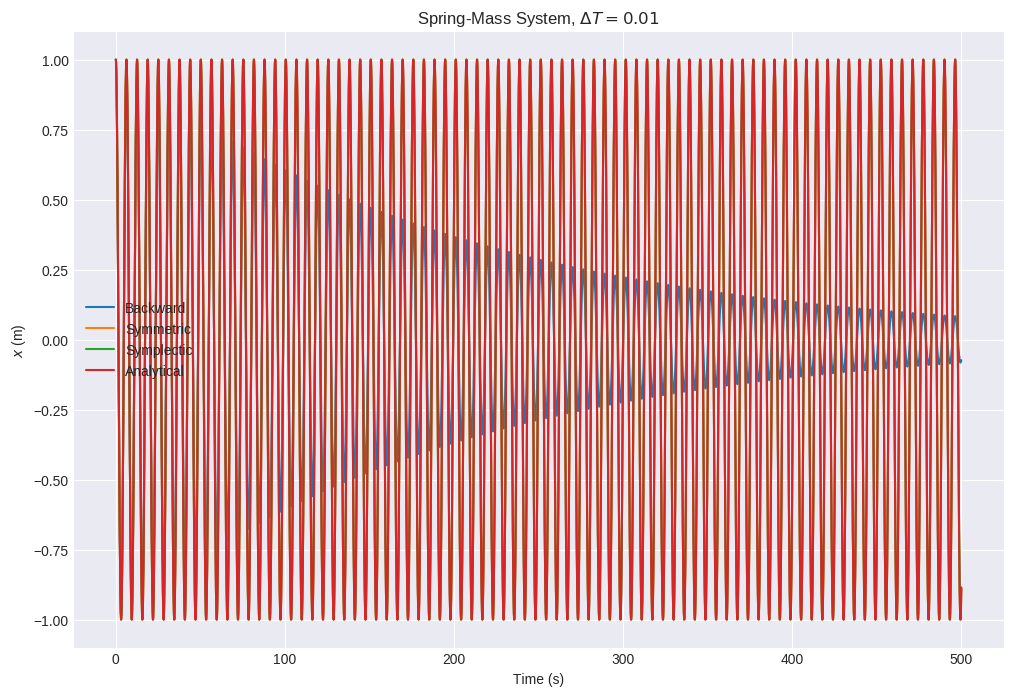
\includegraphics[width=\linewidth]{../sm13.png}
            \caption*{Position vs Time}
        \end{subfigure}
        \begin{subfigure}[H]{0.49\linewidth}
            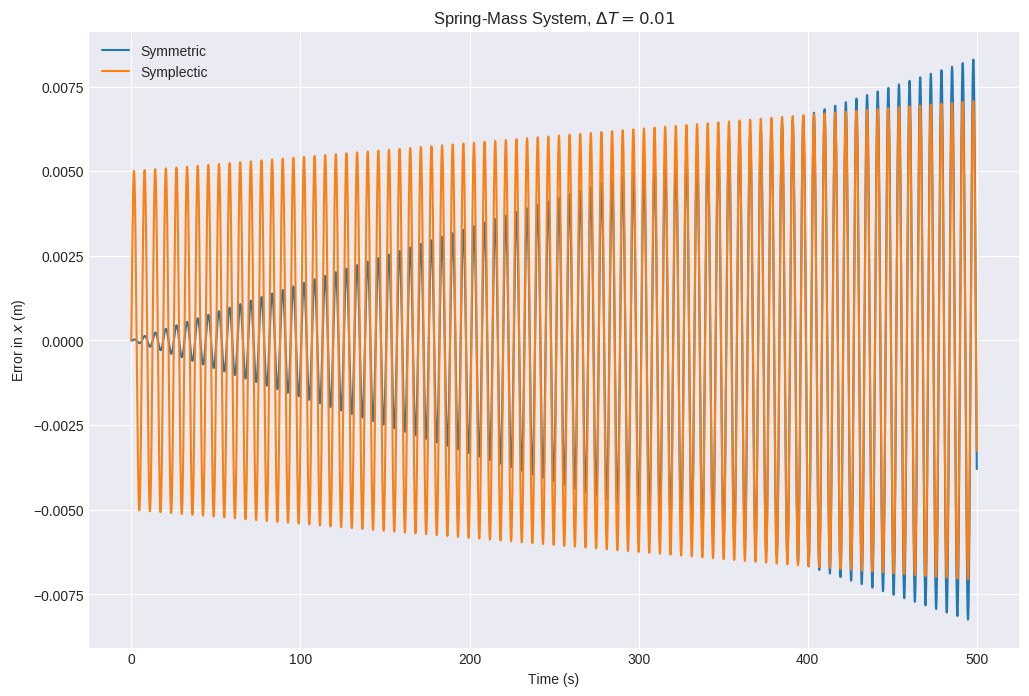
\includegraphics[width=\linewidth]{../sm15.png}
            \caption*{Error vs Time}
        \end{subfigure}
        \caption*{Spring-Mass system, Horizon$ = 500s$}
        \end{figure}

    \begin{figure}[H]
        \centering
        \begin{subfigure}[H]{0.49\linewidth}
            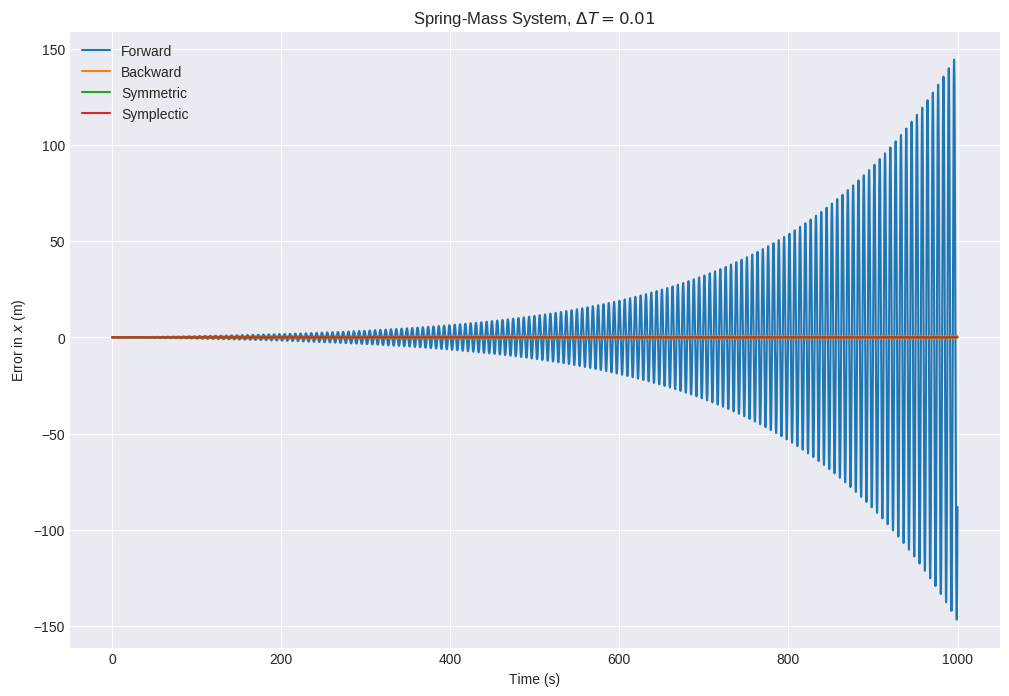
\includegraphics[width=\linewidth]{../sm16.png}
            \caption*{Error vs Time}
        \end{subfigure}
        \begin{subfigure}[H]{0.49\linewidth}
            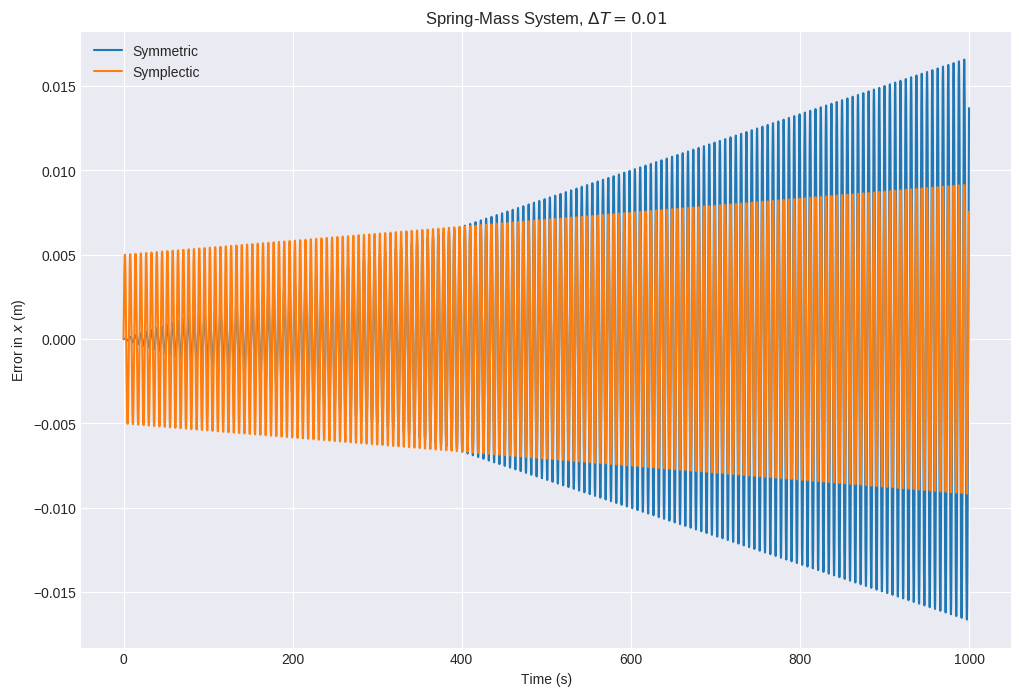
\includegraphics[width=\linewidth]{../sm17.png}
            \caption*{Error vs Time}
        \end{subfigure}
        \caption*{Spring-Mass system, Horizon$ = 1000s$}
        \end{figure}

\subsection*{Vertical Pendulum system}
\begin{figure}[H]
    \centering
    \begin{subfigure}[H]{0.49\linewidth}
        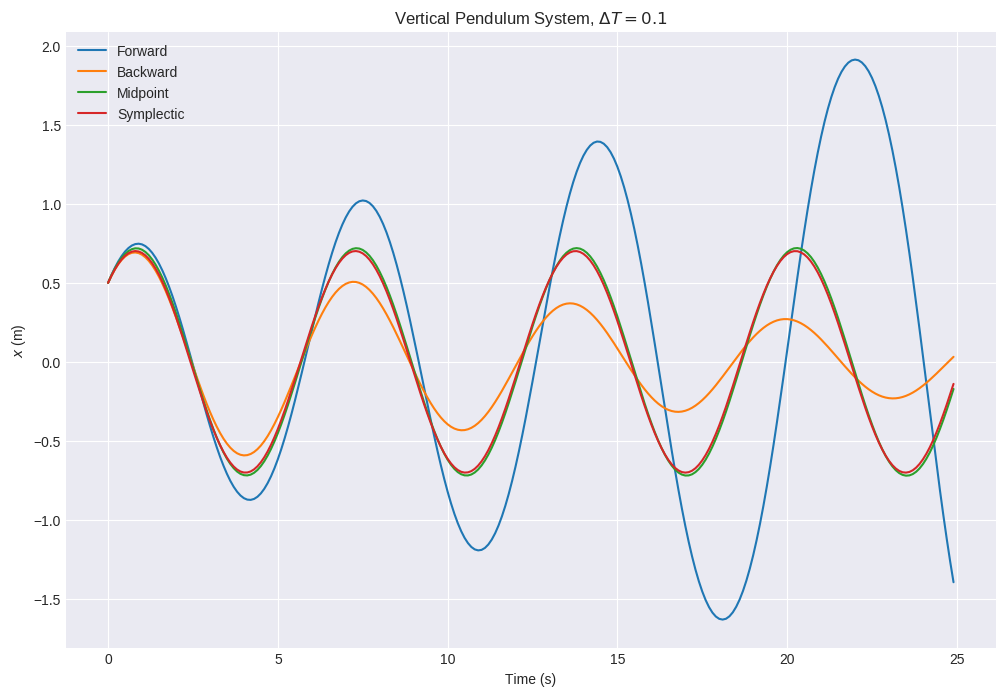
\includegraphics[width=\linewidth]{../vp1.png}
        \caption*{$\Delta T = 0.1s$}
    \end{subfigure}
    \begin{subfigure}[H]{0.49\linewidth}
        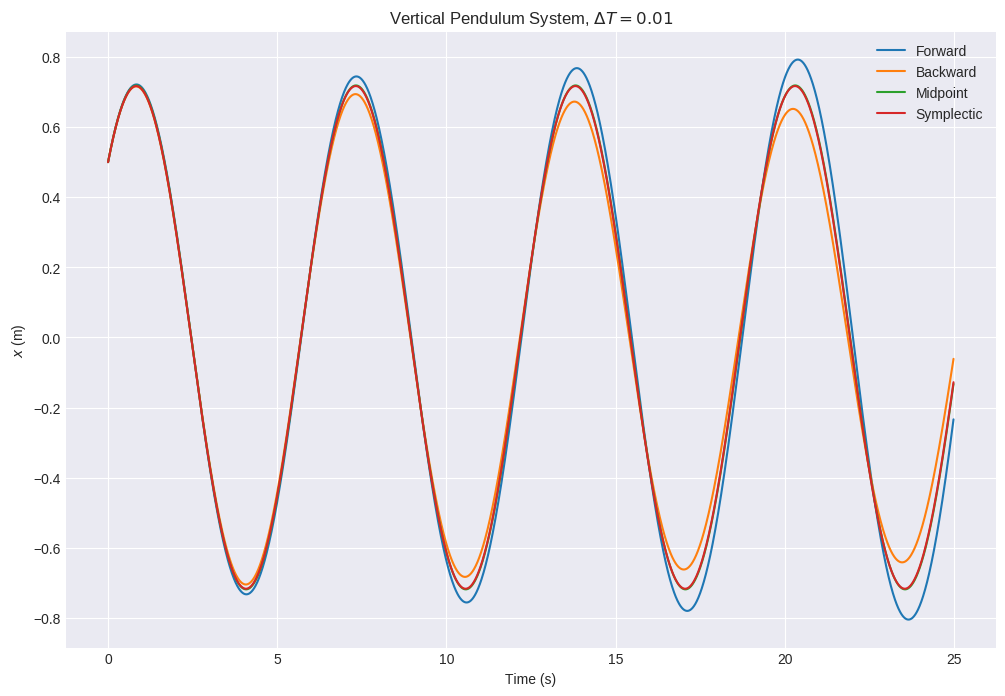
\includegraphics[width=\linewidth]{../vp2.png}
        \caption*{$\Delta T = 0.01s$}
    \end{subfigure}
    \caption*{Vertical Pendulum system, Angle vs Time}
\end{figure}
\begin{figure}[H]
    \centering
    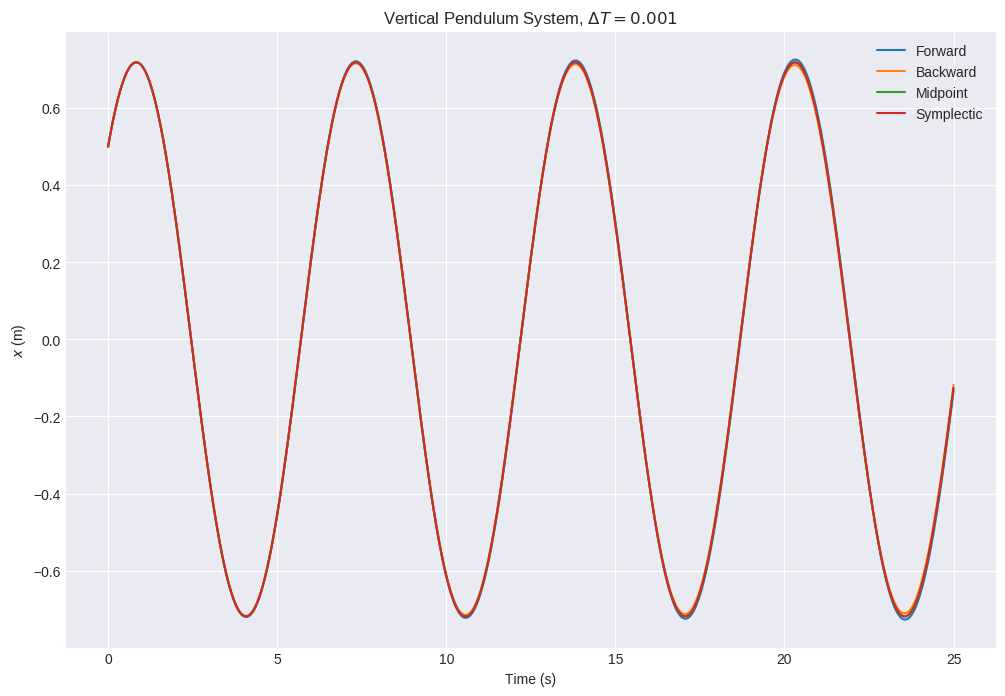
\includegraphics[width=\linewidth]{../vp3.png}
    \caption*{Vertical Pendulum system, Angle vs Time}
\end{figure}

\begin{figure}[H]
    \centering
    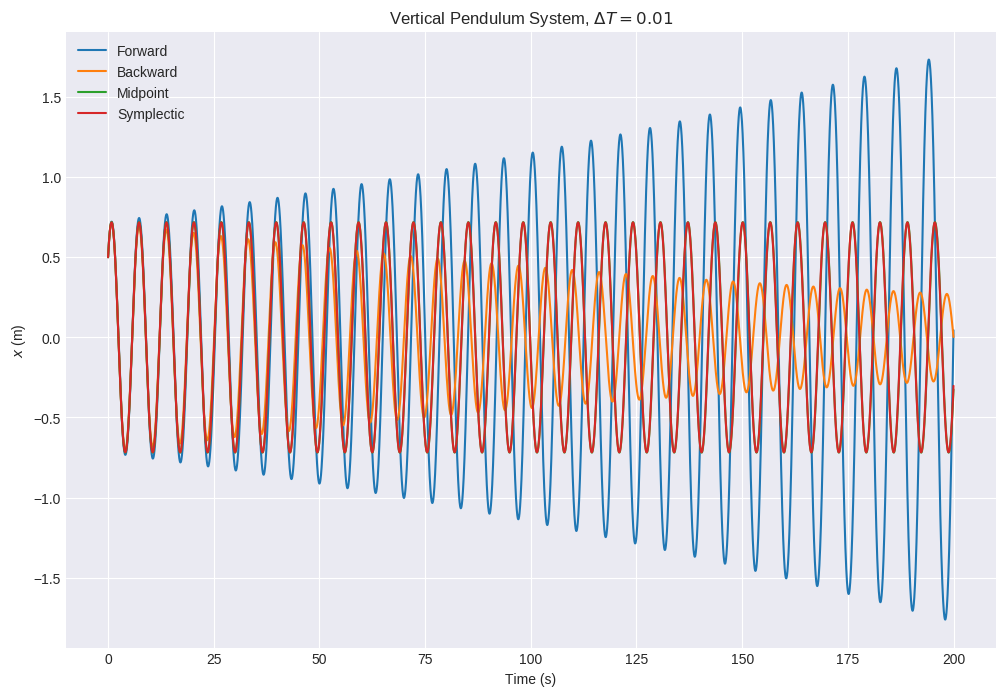
\includegraphics[width=\linewidth]{../vp4.png}
    \caption*{Vertical Pendulum system, Angle vs Time}
\end{figure}

\begin{figure}[H]
    \centering
    \begin{subfigure}[H]{0.49\linewidth}
        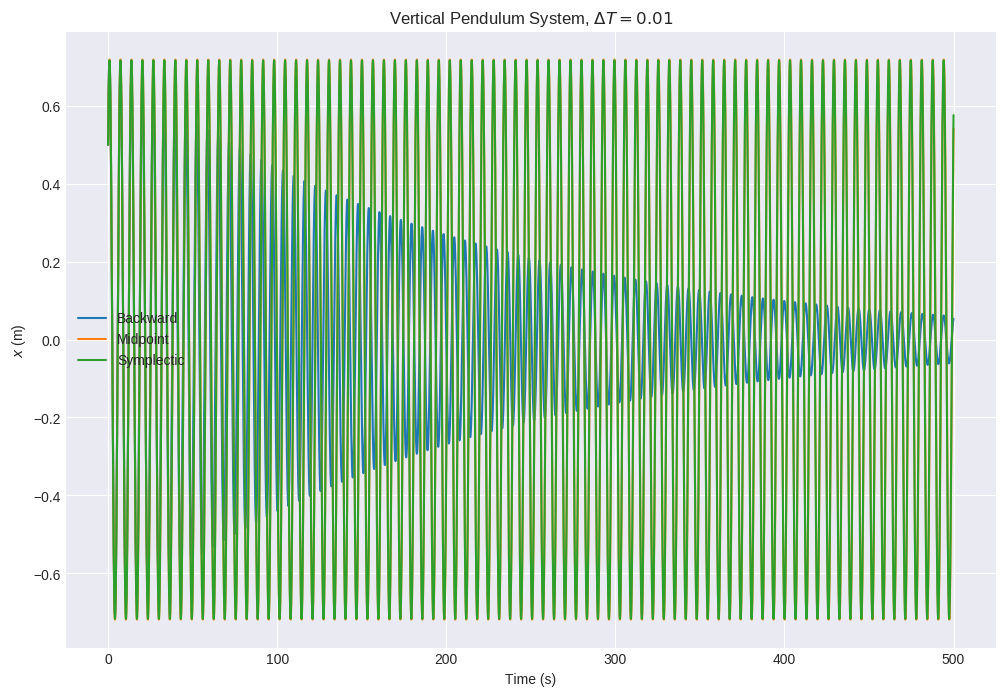
\includegraphics[width=\linewidth]{../vp6.png}
        \caption*{Horizon $ = 500s$}
    \end{subfigure}
    \begin{subfigure}[H]{0.49\linewidth}
        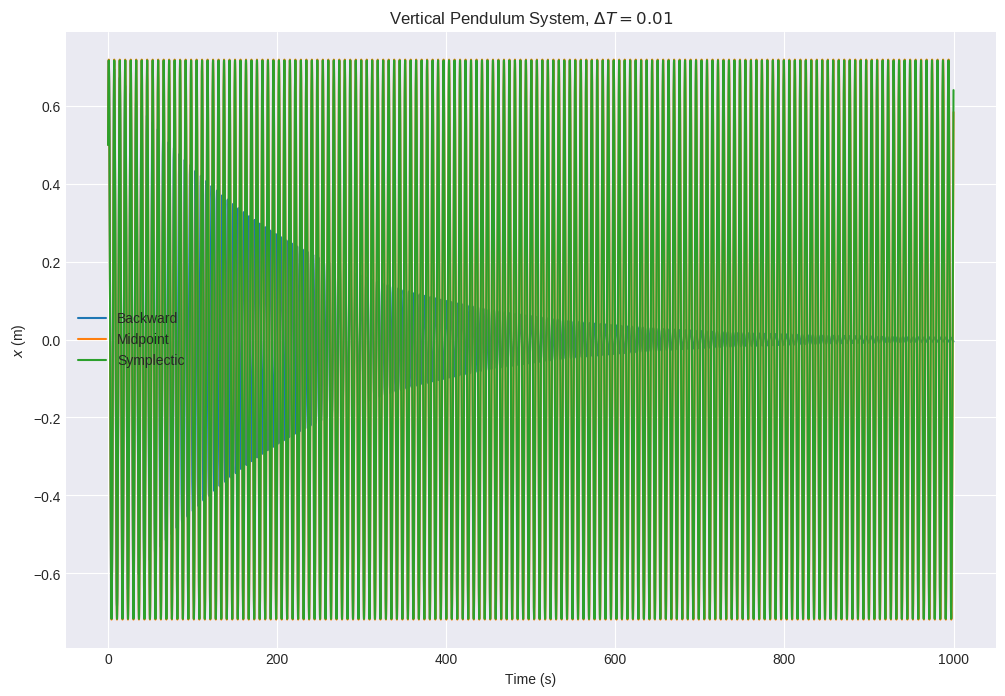
\includegraphics[width=\linewidth]{../vp7.png}
        \caption*{Horizon $ = 1000s$}
    \end{subfigure}
    \caption*{Vertical Pendulum system, Angle vs Time}
\end{figure}

The relative performances of the numerical methods is the same for even the pendulum system. Forward and Backward Euler quickly move away from 
the expected sinusoidal solution. This does not happen with Symmetric and Symplectic Euler.
\section{Kalman Filter}
I simulated the following discrete dynamical system, 
    $$ \mathbf{x_{k+1}} = F \mathbf{x_k} + w_k, \hspace*{5mm} w_k \sim \mathcal{N}(\mathbf{0}, Q)$$
    $$\mathbf{y_k} = H \mathbf{x_k} + v_k, \hspace*{5mm} v_k \sim \mathcal{N}(\mathbf{0}, R)$$

Where $F = \begin{pmatrix}
    1 & \Delta T \\ 0 & 1    
\end{pmatrix}$ , $H = \begin{pmatrix}
    1 & 0
 \end{pmatrix}$
 and $\mathbf{x_k} = \begin{bmatrix}
    x \\ \dot{x}
 \end{bmatrix}$. For the simulation, I used $\Delta T = 0.01s$, $Q = \begin{pmatrix}
    20 & 0 \\ 0 & 20
 \end{pmatrix}$, $R = \begin{pmatrix}
    10
 \end{pmatrix}$. The plots mention the parameters used by the \textbf{Kalman filter}. 

 \begin{figure}[H]
    \centering
    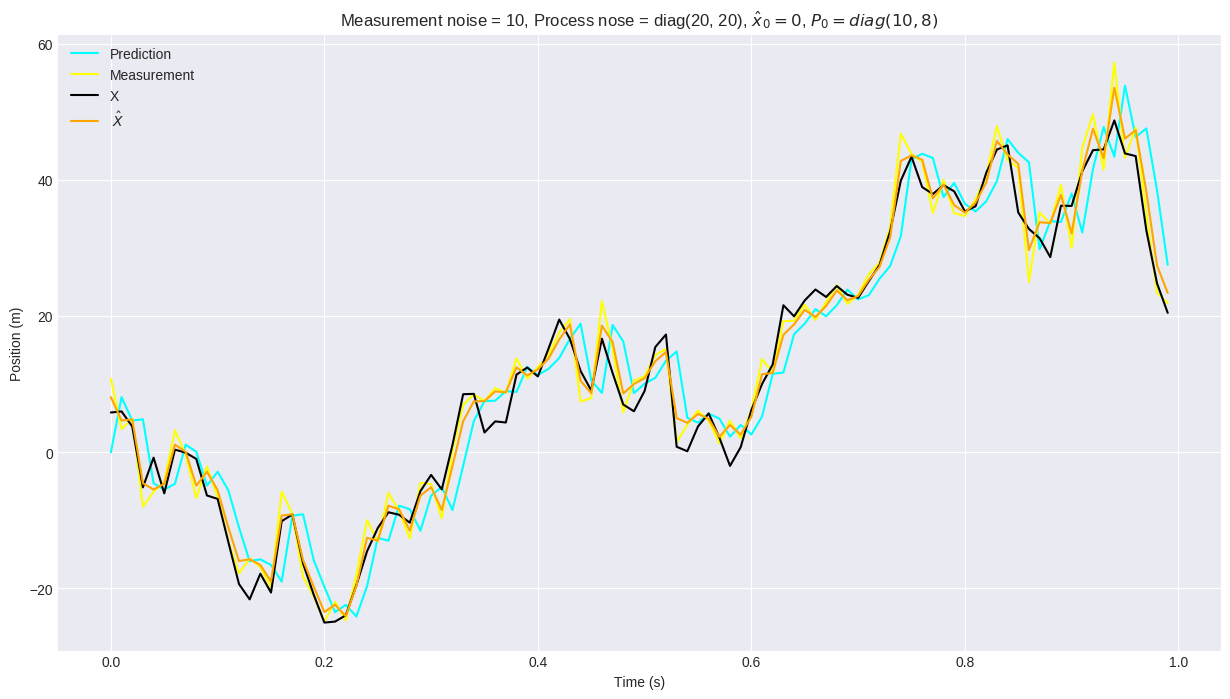
\includegraphics[width=\linewidth]{../kfnormal.png}
    \caption*{Kalman filter}
\end{figure}
The above plot is an ideal situation when the model noise covariances and state-transition, measurement matrices are same as that
of the original system. The estimate is close to the true value of the position of the cart.

However 
in a more realistic situation, the system matrices used in our model will be innacurate and the noise covariances cannot be determined exactly.
The filter still turns out to be robust enough to perform well under these circumstances. It can be seen from the graph 
below that model uncertainties lead to the prediction deviating from the true value of $x$ but the Filter estimates are still close to 
the true value.

It is clearly noticeable how the Filter
responds to changes in the $Q$ and $R$ matrices. Increasing the process-noise covariance causes 
the estimate to lie closer to the measurements and vice-versa. 

The Filter also recovers from large 
initial uncertainties quickly as can be seen in the graph below.
\subsection*{Uncertainty in the model}
\begin{figure}[H]
    \centering
    \begin{subfigure}[H]{0.49\linewidth}
        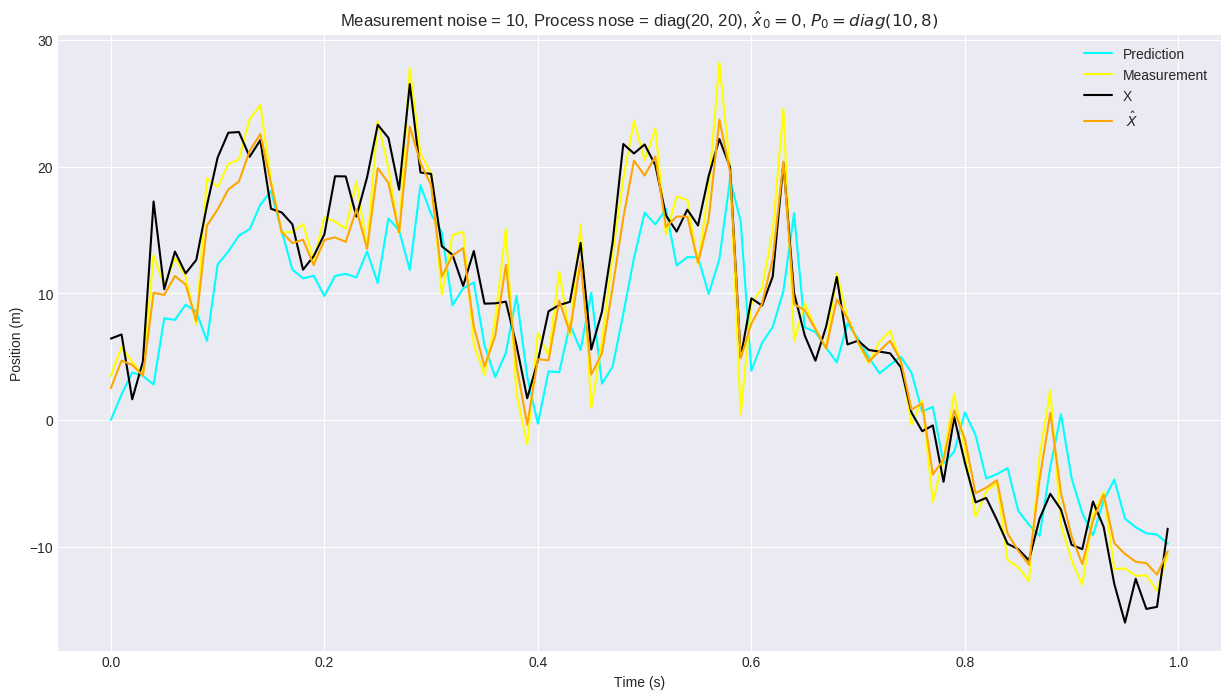
\includegraphics[width=\linewidth]{../kfmodeluncer1.png}
    \end{subfigure}
    \begin{subfigure}[H]{0.49\linewidth}
        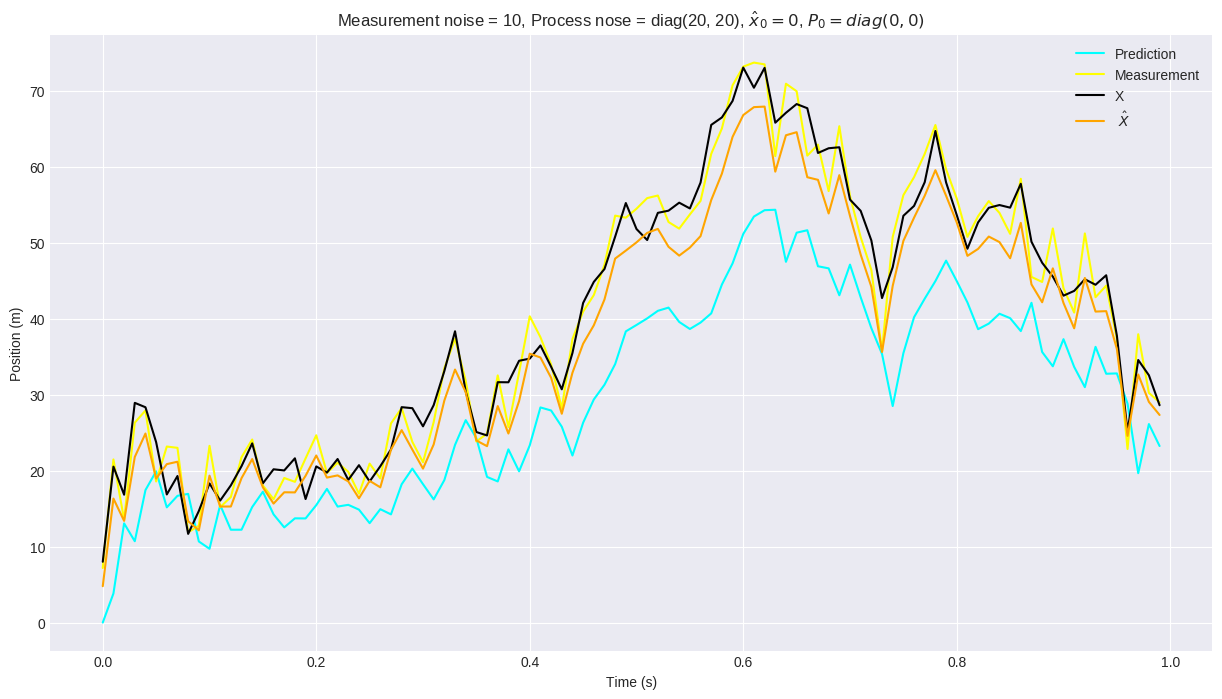
\includegraphics[width=\linewidth]{../kfmodeluncer2.png}
    \end{subfigure}
    \caption*{Uncertain model for two different initial error covariances}
\end{figure}
\subsection*{Tuning the covariances}
\begin{figure}[H]
    \centering
    \begin{subfigure}[H]{0.49\linewidth}
        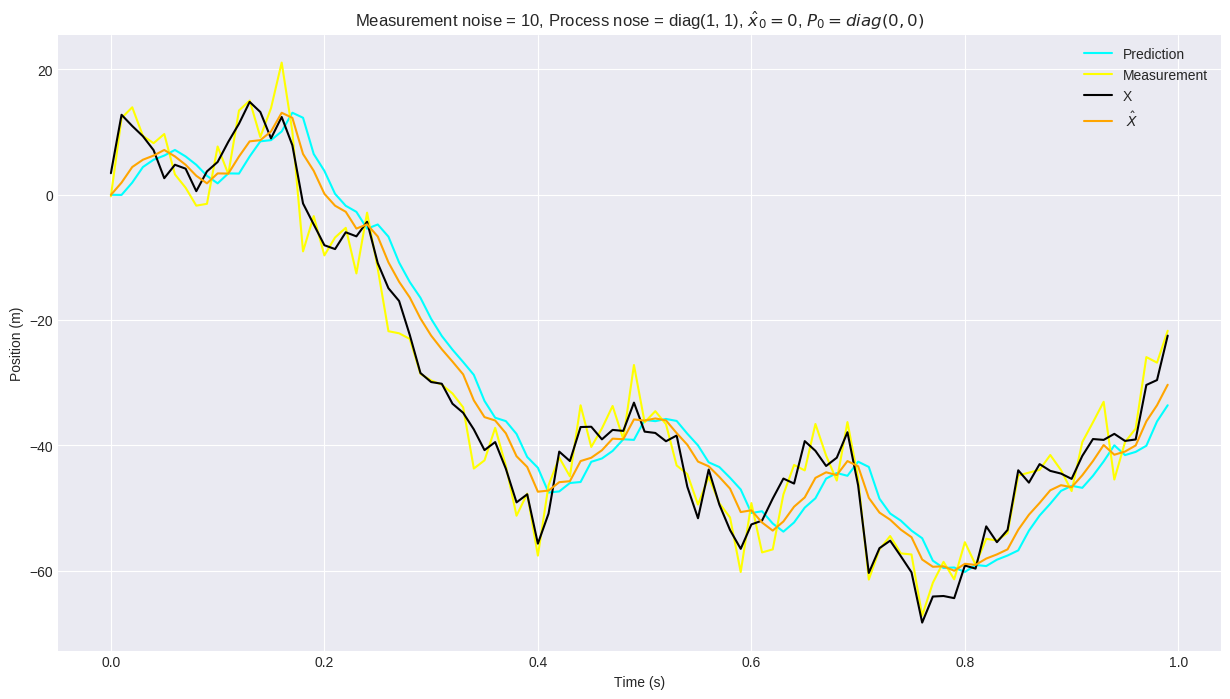
\includegraphics[width=\linewidth]{../kfcov1.png}
        \caption*{High measurement noise}
    \end{subfigure}
    \begin{subfigure}[H]{0.49\linewidth}
        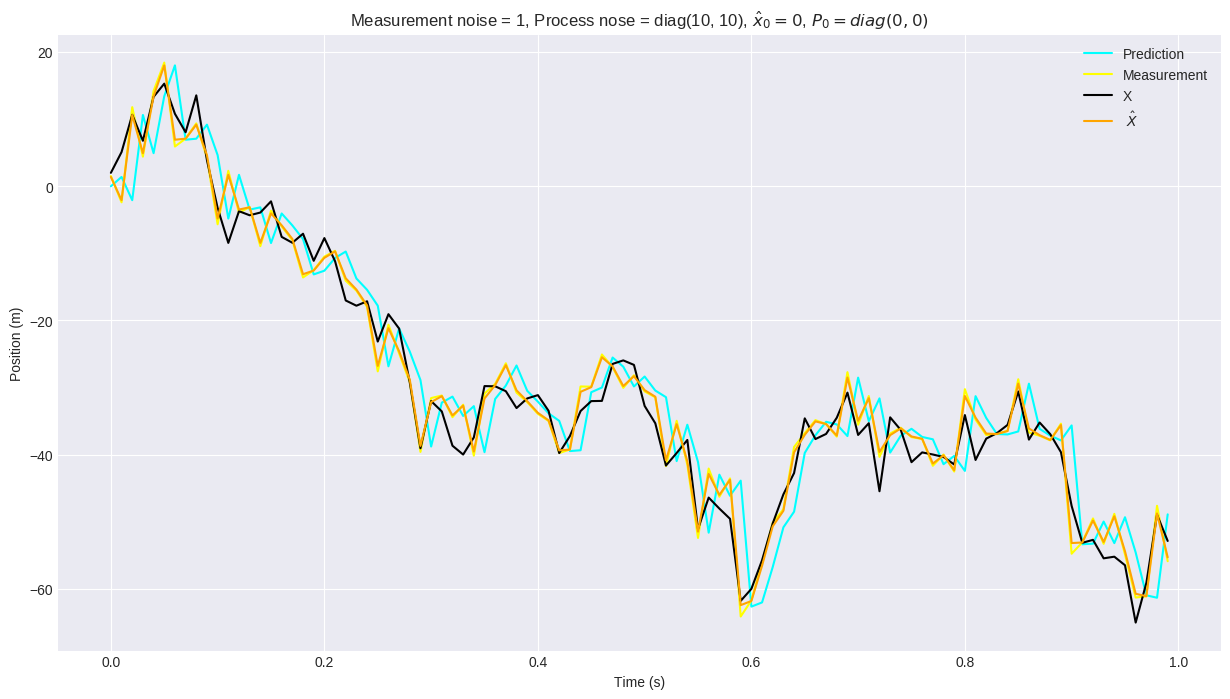
\includegraphics[width=\linewidth]{../kfcov2.png}
        \caption*{High process noise}
    \end{subfigure}
    \caption*{Tuning process and measurement noises}
\end{figure}
Here it is evident that for a high value of the measurement noise variance set in the filter, the estimate is closer to the prediction. 
Similarly for high values of process noise variance, the estimate is closer to the measurement. 
\begin{figure}[H]
    \centering
    \begin{subfigure}[H]{0.49\linewidth}
        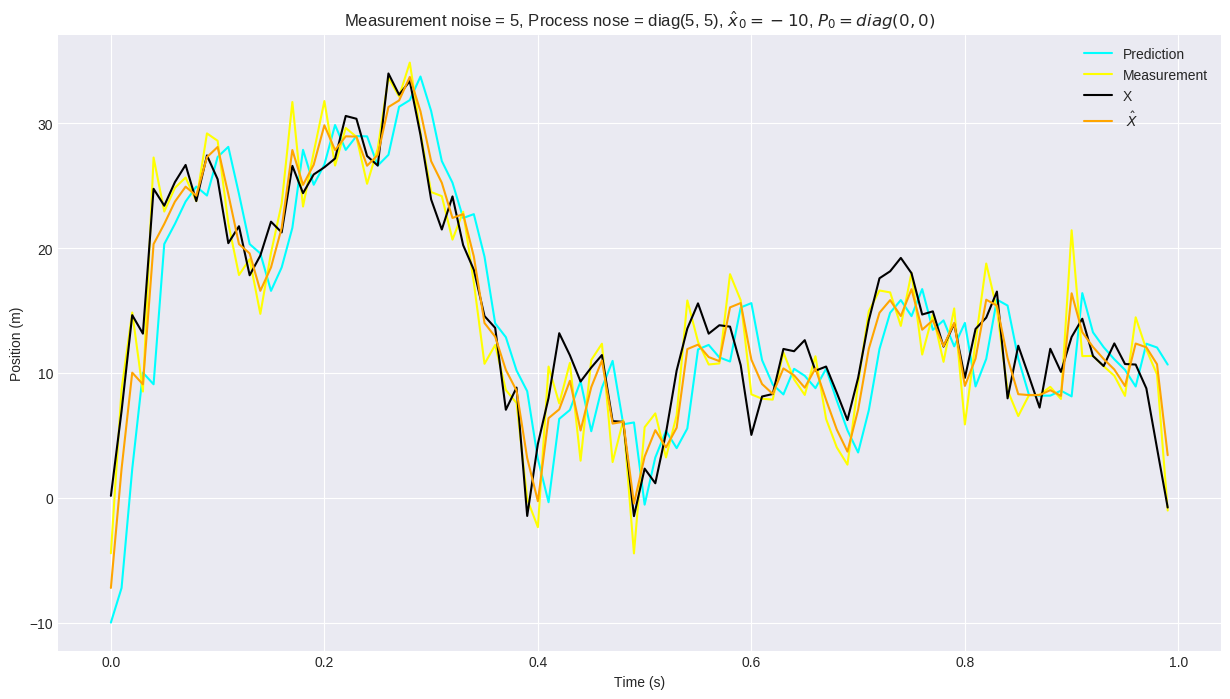
\includegraphics[width=\linewidth]{../kfcov3.png}
        \caption*{High initial error variance}
    \end{subfigure}
    \begin{subfigure}[H]{0.49\linewidth}
        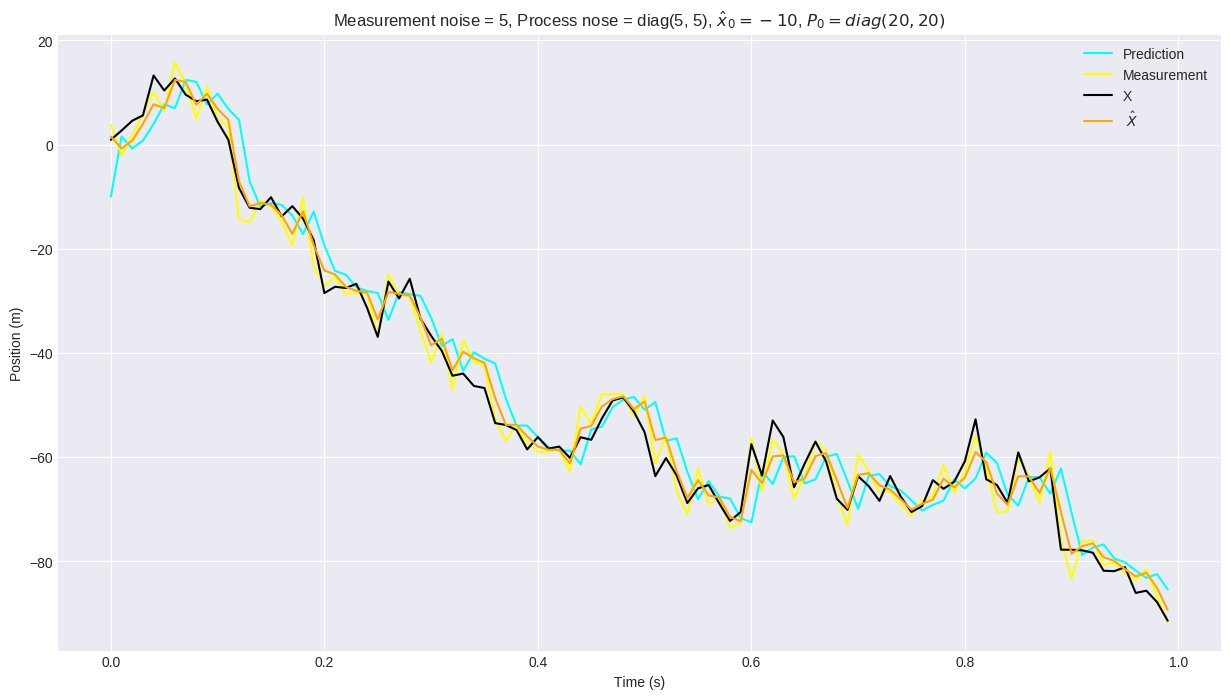
\includegraphics[width=\linewidth]{../kfcov4.png}
        \caption*{Low initial error variance}
    \end{subfigure}
    \caption*{Tuning initial state covariance}
\end{figure}
When the initial error covariance is low, the filter trusts the initial value of $x_0$ more and thus
takes more time to converge to the true value as can be seen from the graph. 

\subsection*{Large initial state uncertainty}
\begin{figure}[H]
    \centering
    \begin{subfigure}[H]{0.49\linewidth}
        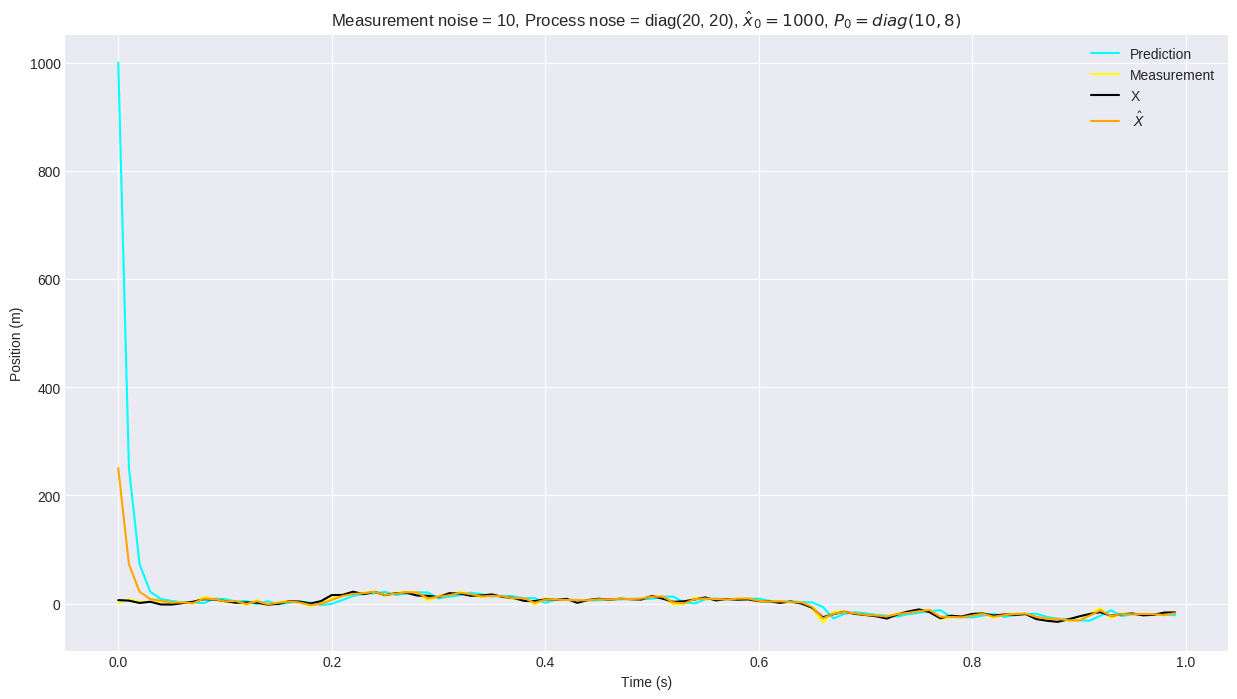
\includegraphics[width=\linewidth]{../kfinituncer1.png}
        \caption*{Quickly recovers}
    \end{subfigure}
    \begin{subfigure}[H]{0.49\linewidth}
        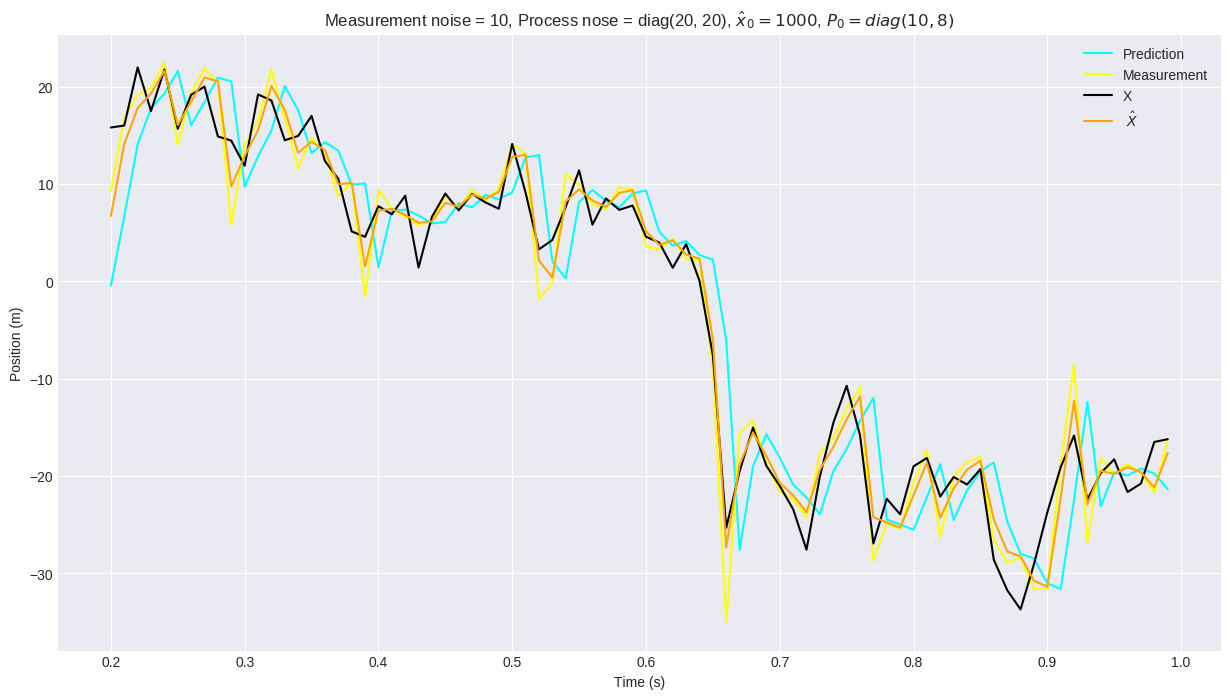
\includegraphics[width=\linewidth]{../kfinituncer2.png}
        \caption*{Zoomed in}
    \end{subfigure}
    \caption*{High initial uncertainty}
\end{figure}

\section{Observer for linear dynamical system}

We keep a proxy of the system along with the state $\hat{x}$ and update it according to our model
of the system and also a correction term as shown below. 

\begin{equation}
    \dot{x} = Ax  \text{ \hspace*{1cm}}
\end{equation}
\begin{equation}
    y = Cx  \text{ \hspace*{1cm}}
\end{equation}
\begin{equation}
    \dot{\hat{x}} = A \hat{x} + L(y - C\hat{x})
\end{equation}

Equations (1) and (2) represent the true system and (3) is our model of the system, where $L(y - C\hat{x})$
is the correction term. $\hat{x}$ is our estimate for $x$ and we can show that $\hat{x}$ converges to
$x$ in the following manner, 
\begin{equation}
    \dot{\hat{x}} = A \hat{x} + LC(x - \hat{x})
\end{equation}
We get (4) by substituting (2) in (3). Now subtract (4) from (1) and define $e \triangleq x - \hat{x} $
\begin{equation}
    \dot{e} = (A - LC)e
\end{equation}
If $(A, C)$ pair is controllable, we can choose an L such that $(A - LC)$ is Hurwitz. 

\end{document}
 